\documentclass[12pt,a4paper]{article}
\usepackage[parfill]{parskip}
\usepackage{fullpage}
\usepackage{enumitem}
\usepackage{hyperref}
\usepackage{graphicx}
\usepackage{subfig}
\usepackage{amsmath}
\usepackage{float}
\usepackage[section]{placeins}

\begin{document}

\vfil

\begin{center}
	{\Large Mobile Robot Systems} \\
	\vspace{0.4in}
	{\huge \bf Assignment 2} \\
	\vspace{0.4in}
	{\large Anik Roy (ar899)} \\
	\vspace{0.1in}
	{\large \today} \\
\end{center}
\vspace{0.4in}

% Main document

\section*{1.1 Potential Field Method}
\subsection*{Exercise 1}
\begin{enumerate}[label=(\alph*)]
	\item The plot of the potential field for moving towards the goal can be seen in figure \ref{fig:goal_mode}. This field is calculated by taking the vector from the position towards the goal, and squaring the magnitude of the vector while keeping the same direction. This ensures that the robot 'slows down' as it gets closer to the goal, and that it will always attempt to move towards the goal. The figure shows how all the vectors point towards the goal, and that vectors close to the goal have a smaller magnitude. Squaring the magnitude also allows it to have a smoother decrease in speed than if it was linear.
	\begin{figure}[!htb]
		\centering
		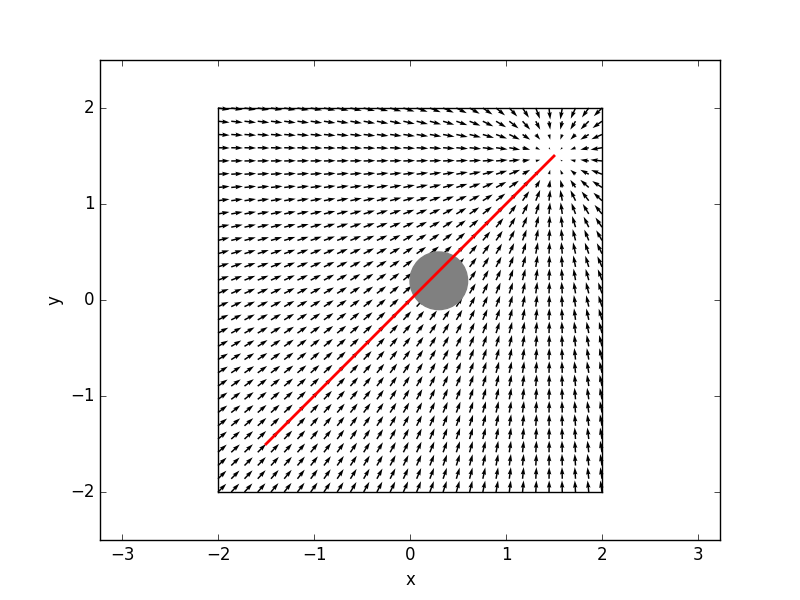
\includegraphics[width=12cm]{fig/1a.png}
		\caption{Potential field with the goal}
		\label{fig:goal_mode}
	\end{figure}
	\item In order to avoid obstacles, we also need to find a vector field which will let us move away from obstacles (a field that is repulsive). In order to do this, I first find the distance from the position to the surface of the  obstacle by finding the euclidean distance and subtracting the radius. Since positions closer to the obstacle should be more 'repulsive', the reciprocal of this distance is the magnitude of the final vector. The direction of the final vector is directly away from the centre of the obstacle towards the robot. I also scale this by a tunable parameter to ensure the robot makes progress. Without scaling, the repulsion would be too strong or too weak, meaning the robot would either take too long to get to the goal or not get there at all. This process is repeated for each obstacle, and the vectors produced are summed so that all the obstacles are taken into account. The resulting vector is also capped to a maximum speed.
	\begin{figure}[!htb]
		\centering
		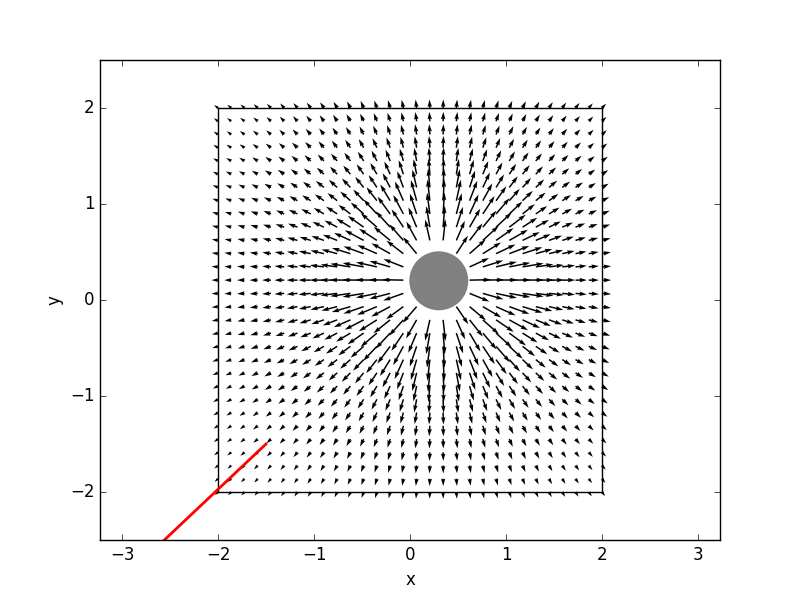
\includegraphics[width=12cm]{fig/1b.png}
		\caption{Potential field with the obstacles}
		\label{fig:obs_mode}
	\end{figure}
	\item Figure \ref{fig:all_mode} shows how combining the two vector fields results in a new field which allows the robot to take a path to the goal while avoiding the obstacle. Since the vectors from the obstacle have a repulsive effect, and the vectors towards the goal have an attactive effect, they combine these effects to create vectors which go towards the goal but also away from the obstacle.
	\begin{figure}[!htb]
		\centering
		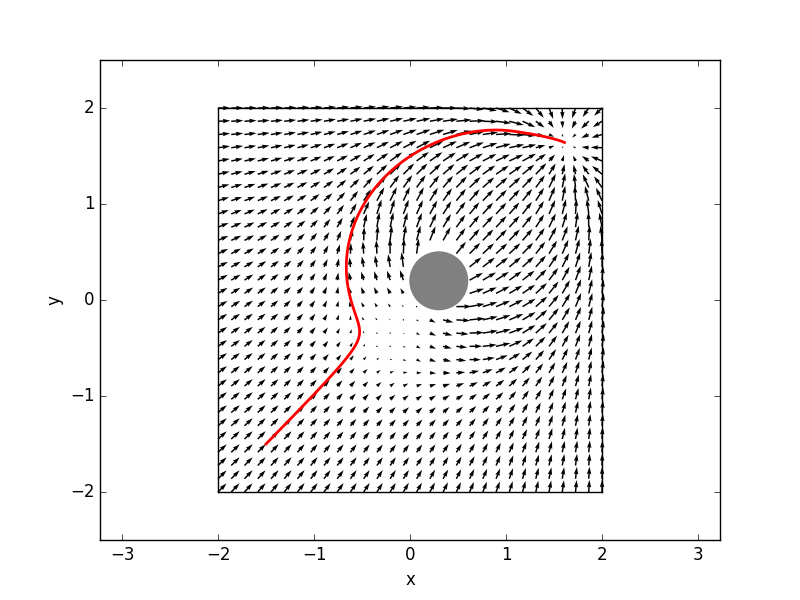
\includegraphics[width=12cm]{fig/1c.png}
		\caption{Potential field with both the goals and the obstacle}
		\label{fig:all_mode}
	\end{figure}
	\item In the previous part, the obstacle was at the position (0.2,0.3). Since the robot started at (-1.5,-1.5), and the vectors for the goal are direct, they will pass directly through the center of the obstacle. The vectors from the obstacle are in the opposite direction, as the direction of these vectors is the direction from the robot to the obstacle flipped. This means they will cancel each other out to produce a zero vector somewhere between the start position and the obstacle, stopping the robot. This can be seen in \ref{fig:failed_potential}, where the robot gets stuck halfway between the start and the obstacle. The area which looks more empty is the local minimum that the robot `falls' into. One possible solution is to change the direction of the vectors coming from the obstacle. Currently, they are directly in the direction of the robot, but they could be made to be skewed slightly so that the robot would always move in one direction. Once the robot moves in the direction, vectors towards the goal should allow the robot to keep moving. This still ensures the robot does not hit the obstacle, since the vectors are still repulsive, just in a slightly different direction.
	\begin{figure}[!htb]
		\centering
		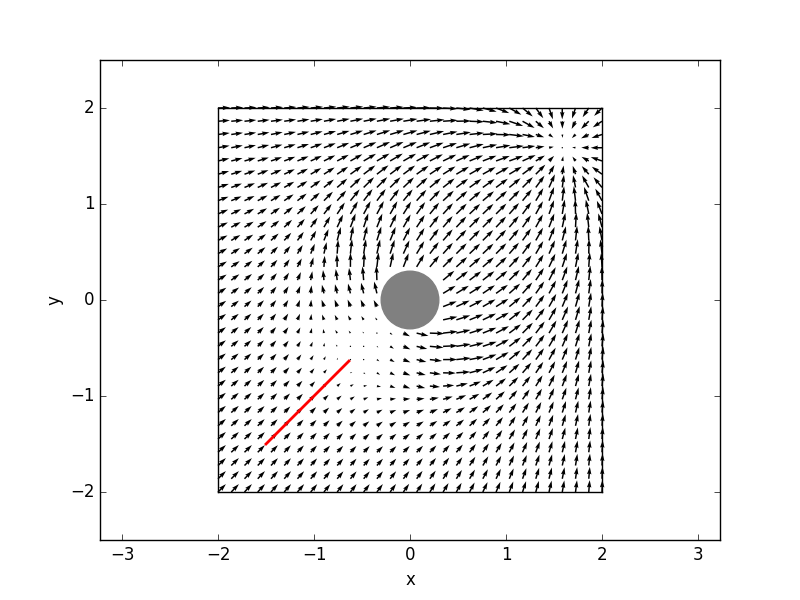
\includegraphics[width=12cm]{fig/1d.png}
		\caption{Potential field with the obstacle at (0,0)}
		\label{fig:failed_potential}
	\end{figure}
	\item Figure \ref{fig:fixed_potential} shows how the problem in part (d) can be fixed. The vectors coming from the obstacle are now rotated by 1 radian anti-clockwise (which can be tuned). This means that the robot will now take the path on the right of the obstacle, as it is pushed in that direction by these vectors. To calculate the vectors, I use the standard 2-D rotation matrix to ensure that the magnitude of the vector stays the same (it is rotated from its original direction around its base).
	\begin{figure}[H]
		\centering
		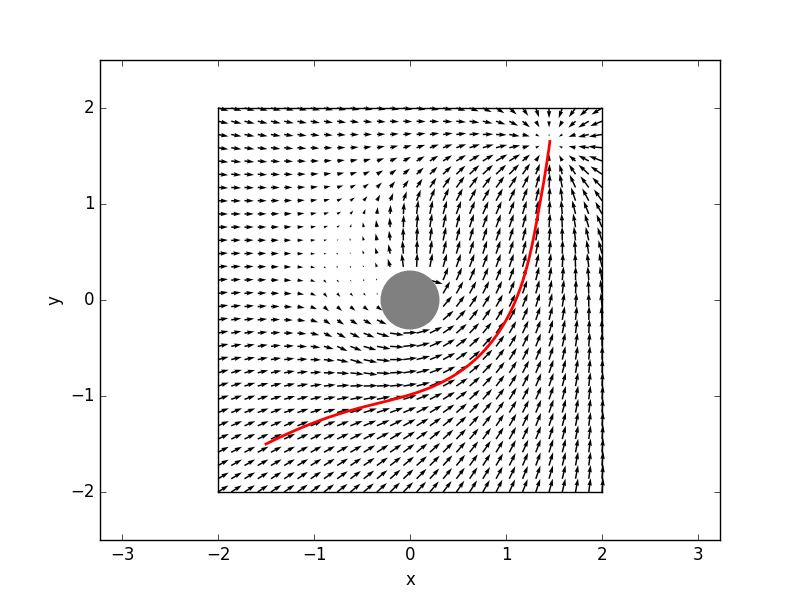
\includegraphics[width=12cm]{fig/1e.png}
		\caption{Potential field with the obstacle at (0,0), fixed}
		\label{fig:fixed_potential}
	\end{figure}
	\item The solution from part (e) still works with two obstacles, with the robot taking a similar path as it is repulsed from both the obstacles.
	\begin{figure}[H]
		\centering
		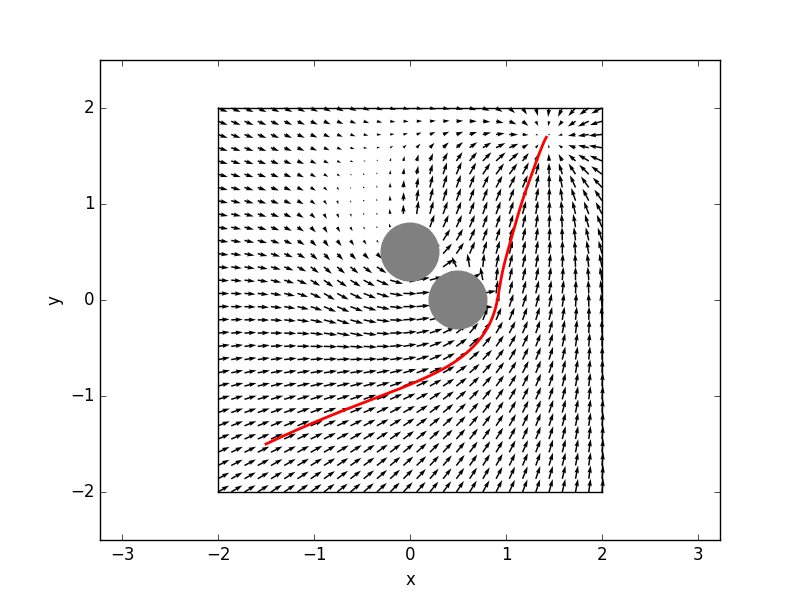
\includegraphics[width=12cm]{fig/1f.png}
		\caption{Potential field with two obstacles at (0,0.5) and (0.5,0)}
		\label{fig:fixed_potential}
	\end{figure}
	
\end{enumerate}
\subsection*{Exercise 2}
\begin{enumerate}[label=(\alph*)]
	\item The equations for feedback linearization:
		$$\dot{x_p} = u\cos{\theta} - \epsilon \omega \sin{\theta}$$
		$$\dot{y_p} = u\sin{\theta} + \epsilon \omega \cos{\theta}$$
		Rearranged for $u$ and $\omega$:
		$$ u =x_p\cos{\theta} + y_p\sin{\theta} $$
		$$ \omega = {(-x_p\sin{\theta}+y\cos{\theta})\over{\epsilon}}$$
	\item The point of feedback linearisation is to allow a non-holonomic robot to move in the same trajectory as a holonomic point, by controlling a holonomic point and calculating how the robot would move as if 'pulled' by that point. We can choose the trajectory of the holonomic point to be any path, but without feedback linearization it would be hard to find values of $u$ and $\omega$ (and therefore speeds for the two wheels) which would actually move the robot along that path. More generally, feedback linearization allows a non-linear system (here, the non-holonomic robot following a path) to be transformed into a linear system which can then be controlled as needed.
	\item The plot below shows the trajectory of the robot as it navigates from the start to the goal. The green line shows the trajectory of the holonomic points, with the blue line being the trajectory of the robot following that point. We can see that the two trajectories are approximately the same, showing how feedback linearization allows the non-holonomic robot to move along a holonomic trajectory.
	\begin{figure}[!htb]
		\centering
		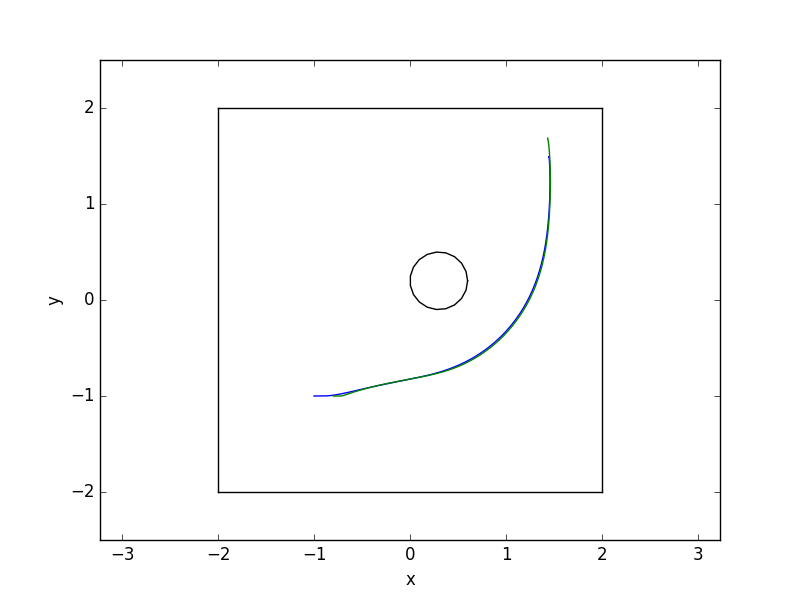
\includegraphics[width=\textwidth]{fig/2c.png}
		\caption{Trajectory of robot in potential field}
		\label{fig:trajectory}
	\end{figure}
	\item There is no reason to need to use the absolute pose of the robot, since we can convert all the points to coordinates relative to the robot and still calculate the same potential field as before. This works since everything is shifted into coordinates relative to the robot, including the entire potential field. For example, the potential at a point in relative coordinates will be the same as the potential at that same point in absolute coordinates - since the position of the cylinder and goal are also relative (and these are the only two other coordinates \texttt{get\_velocity} rely on), the same potential is calculated. This can be very useful in the case that we don't have absolute coordinates to use, e.g. we don't have a complete map of the environment and want to be able to react to new obstacles. For example, if we decided to use an algorithm like SLAM to map out obstacles as the robot moved (which we would then pass to a get\_velocity function), using relative coordinates would be easier since we don't have a full map and it would be easier to find locations relative to the robot. Using relative position also means we don't 
	\begin{figure}[!htb]
		\centering
		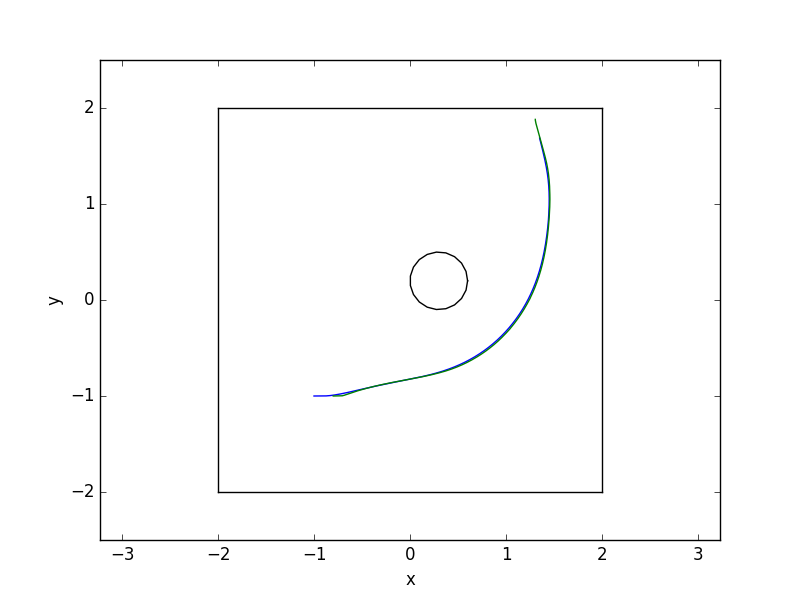
\includegraphics[width=\textwidth]{fig/2d.png}
		\caption{Trajectory of robot in potential field, using relative position}
		\label{fig:trajectory}
	\end{figure}

\end{enumerate}

\section*{1.2 Rapidly-Exploring Random Trees}

\subsection*{Exercise 3}
\begin{enumerate}[label=(\alph*)]
	\item The \texttt{sample\_random\_position} method finds a random position that is not occupied (or unknown) within the occupancy grid. It does this by finding the size of the array (\texttt{grid.values}) backing the grid object, and from this calculating the possible positions in world coordinates that the grid represents. The \texttt{get\_position} method of the grid allows us to find the position encoded by the first (top left, index [0,0]) and last (bottom right, index [len(grid), len(grid[0])]) elements of the occupancy grid. From this we have the set of coordinates we can sample from - we have the maximum and minimum for both x and y coordinated. We then sample uniformly from this range (both x and y), and check if that position is free. We continue sampling until we find a position that is free.
	\item The method of Rapidly exploring Random Trees (RRT) is used to plan a path to the goal. This method samples random points in the free space and attempts to connect the point to other points to build up a tree which explores the area of the free space. Figure \ref{fig:rrt} shows paths generated by my rrt method. The texttt{adjust\_pose} method takes a start node and a final position. It then returns a node which has the final position and a yaw that corresponds to an arc between the start node and the final position. It returns none if this arc collides with something in the occupancy grid. First, we find the yaw of the final node, which is equal to $2 \cdot \theta - yaw$, where $\theta$ is the angle of the vector between the two nodes. This gives us an arc with the yaw of both endpoints being tangent to the circle. Using the texttt{find\_circle} method, we find the centre and radius. To check for collisions, we find the angle and length of the arc. Since we want to be sure that every value in the grid on the arc is sampled, we make sure to step along the arc in increments of the resolution. Using the vector from the centre to the arc, I sample points along the arc and check they are free in the occupancy grid, returning \texttt{None} if there is any point that isn't free.	
	\begin{figure}[h!]
		\centering
		\subfloat{{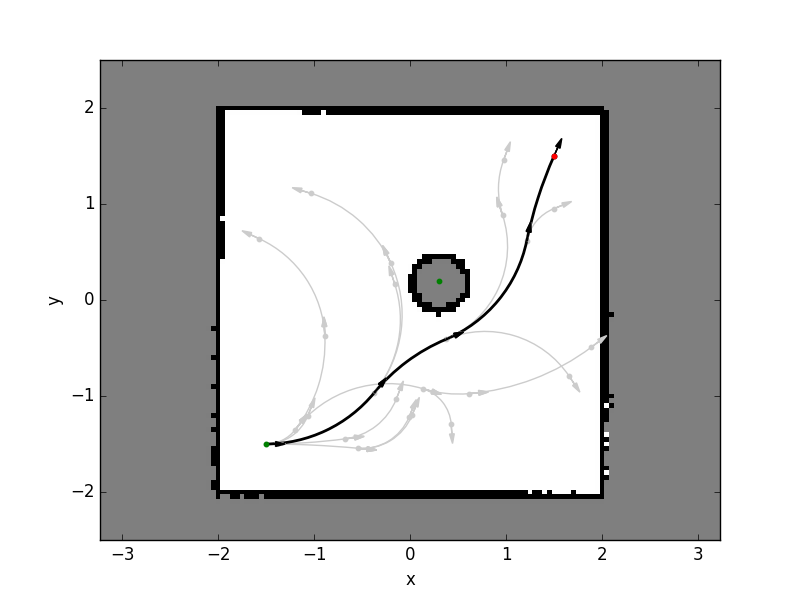
\includegraphics[width=7cm]{fig/3b.png}}}%
		\qquad
		\subfloat{{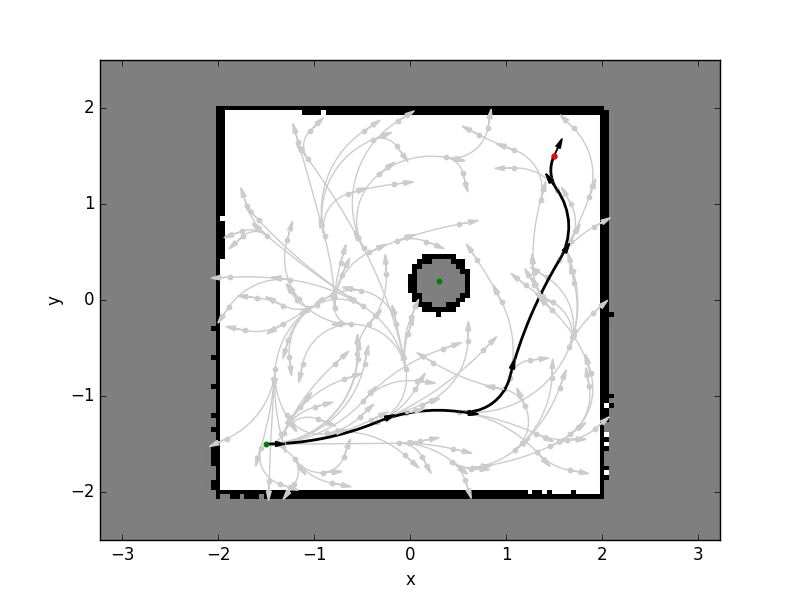
\includegraphics[width=7cm]{fig/3b_1.png}}}%
		\caption{Paths generated by RRT}		
		\label{fig:rrt}%
		\end{figure}

	\item RRT will often find a suboptimal path due to the fact the the random points that are sampled will just be connected to the closest pre-existing node. This closest point may not always be the best point to connect to, since the path to that node may be longer that it needs to be. A solution is to use the RRT* algorithm, accumulating `costs', which represent the distance taken by the shortest path from the root to the node. We can then connect to the nodes with the least cost rather than just the nearest neighbour. We can also carry out a `rewiring' step, which will use the new node generated to find shorter paths for nearby nodes, changing the parent of nearby nodes to the new node if using the new node will reduce the cost to the nearby nodes. This ensures shorter paths are created from the new randomly generated position.
	\item Figure \ref{fig:rrt-star} shows the implementation of RRT* generating shorter and smoother paths. To implement RRT*, I use the `cost' field in the \texttt{Node} class to store the current distance up to that node. When creating a new node, I first take the closest node to get a distance `to beat', then look in a `neighbourhood' - nodes that are within some radius of the new node and in the correct direction. If there is a lower cost node in the neighbourhood, I connect the new point to that node instead (after having adjusted the pose to get the correct direction for this lower cost node). For the rewiring step, I again look in the neighbourhood to find nodes to rewire to the new node. If using the new node gives a lower cost, then I change the parent of the other node to be the newly generated node. I then remove the node from it's parents neighbours to ensure the final path will be the correct lower cost one. This method is much slower that the standard RRT algorithm since it checks a lot more arcs due to the rewiring, but does produce paths which are much smoother and shorter (compared to the more winding paths of RRT) since it looks for paths which are shorter rather than greedily picking the closest node each time.
	\begin{figure}[h!]
		\centering
		\subfloat{{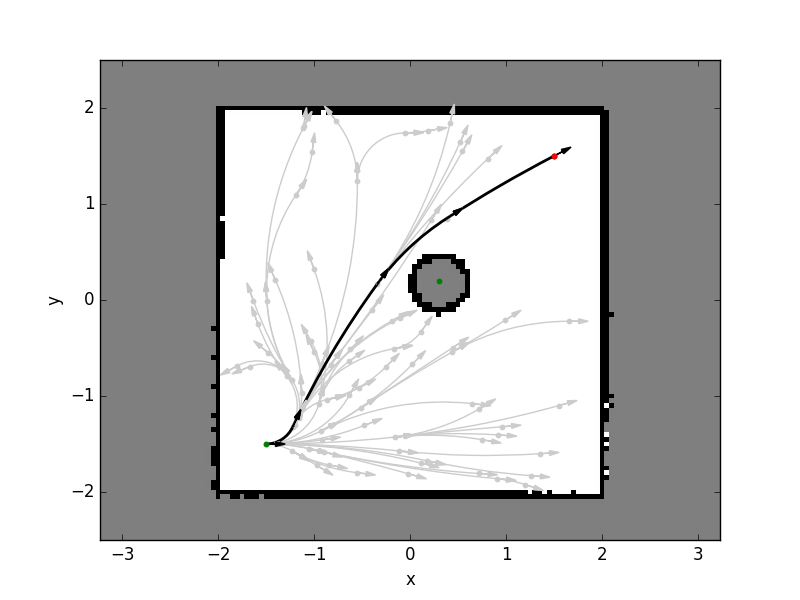
\includegraphics[width=7cm]{fig/3d.png}}}%
		\qquad
		\subfloat{{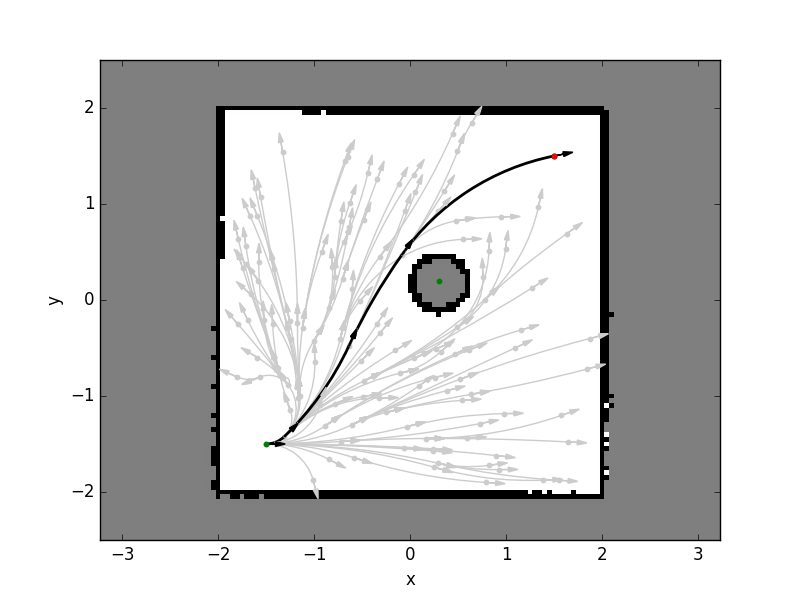
\includegraphics[width=7cm]{fig/3d_1.png}}}%
		\caption{Paths generated by RRT*}		
		\label{fig:rrt-star}%
	\end{figure}

\end{enumerate}
\subsection*{Exercise 4}
\begin{enumerate}[label=(\alph*)]
	\item Feedback linearization is implemented here the same as in exercise 2 (c)
	\item Motion primitives can be used to generate edges for non-holonomic robots. This means we don't have to solve a boundary value problem (set of differential equations) to generate edges which are valid trajectories for non-holonomic robots. However, it does mean that the paths we generate are not always the best paths to take, and we only take into account one (or a few) kinds of motion. In this case, we only take trajectories that are circular arcs, and don't include different types of path such as bezier curves.
	\item The \texttt{get\_velocity} method generates a velocity vector based on a robot position and a set of points which represent the desired trajectory of the robot. First, it finds the point on the path which is closest to the position of the robot. The subsequent point on the path is the direction in which the velocity is, since we want to make sure the robot gets closer to the desired path. If the closest point is the point at the end of the path, then the vector is just in that direction (avoiding the index being out of bounds). Figure \ref{fig:rrt-slam} shows how a path is generated by rrt, which the robot then follows using \texttt{get\_velocity} and \texttt{feedback\_linearized}. The method makes sure that the velocity vector has the same magnitude (the constant speed), and so is a simple bang-bang closed loop controller.
	\begin{figure}[!htb]
		\centering
		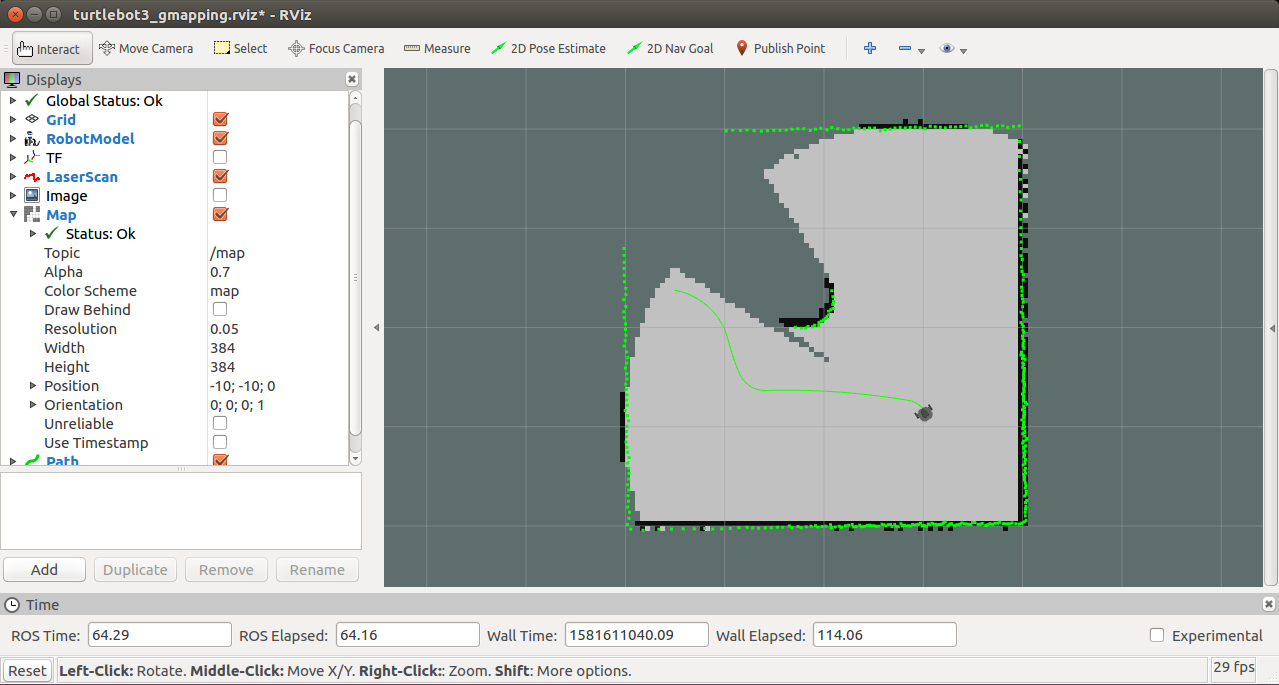
\includegraphics[width=\textwidth]{fig/4c.png}
		\caption{RViz window showing RRT with SLAM}
		\label{fig:rrt-slam}
	\end{figure}
	\item SLAM stands for simultaneous localisation and mapping, and is an algorithm for generating a map of an environment as well as locating where in that map the robot currently is. Running \texttt{roslaunch exercises slam.launch} starts rostopics for the map generated by SLAM, which can be subscribed to for the occupancy grid of all the locations currently known. As the robot explores more area, more of the map gets filled out, generating more values for the occupancy grid. The RRT algorithm needs the occupancy grid to be able to generate valid paths, and it needs the goal to be free in the grid, i.e. it should have been mapped by SLAM. The ro bot will need to move along the trajectory generated by RRT, and will re-generate new trajectories as SLAM maps more of the environment.
	\item The procudure uses the SLAM and RRT algorithms to find a path to some point in the mapped space, which can be specified in the RViz window. The path that is generated by the RRT is followed using the \texttt{get\_velocity} function (bang-bang controller). The path is updated periodically in order to account for new information from SLAM. This continues until the robot reaches the goal position. The enviroment I used to test on the real turtlebot can be seen in figure \ref{fig:environ} - A single rectangular obstacle was placed in the middle of the environment (similar to the cylinder in the simulations). The goal was set to be a position to the side of the box which could be mapped by the robot from the initial position. The RViz windows in figures \ref{fig:before} \ref{fig:during} \ref{fig:after} show the state of the map before, during and after navigation to the goal. The green line shows the path generated by the initial round of RRT.
	\begin{figure}[!htb]
		\centering
		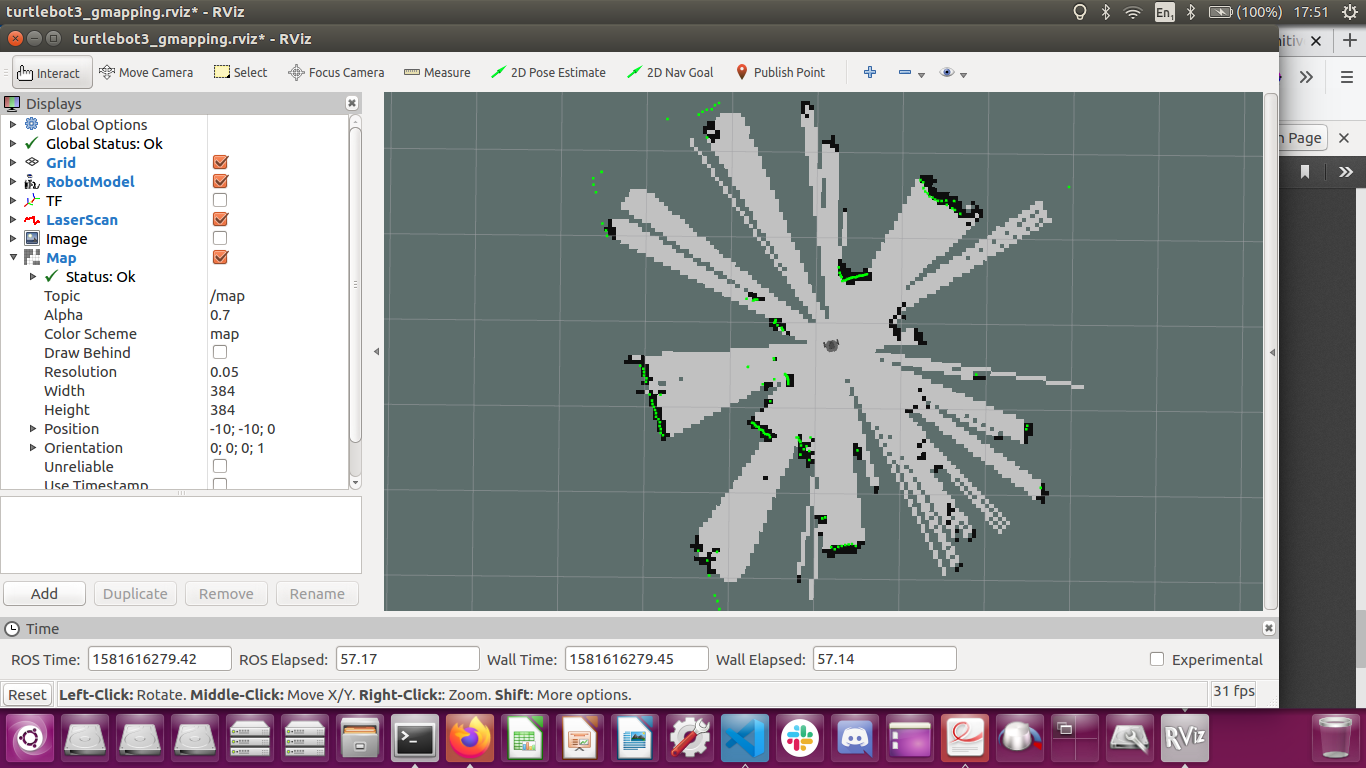
\includegraphics[width=\textwidth]{fig/4e-before.png}
		\caption{The state of the map before moving}
		\label{fig:before}
	\end{figure}

	\begin{figure}[!htb]
		\centering
		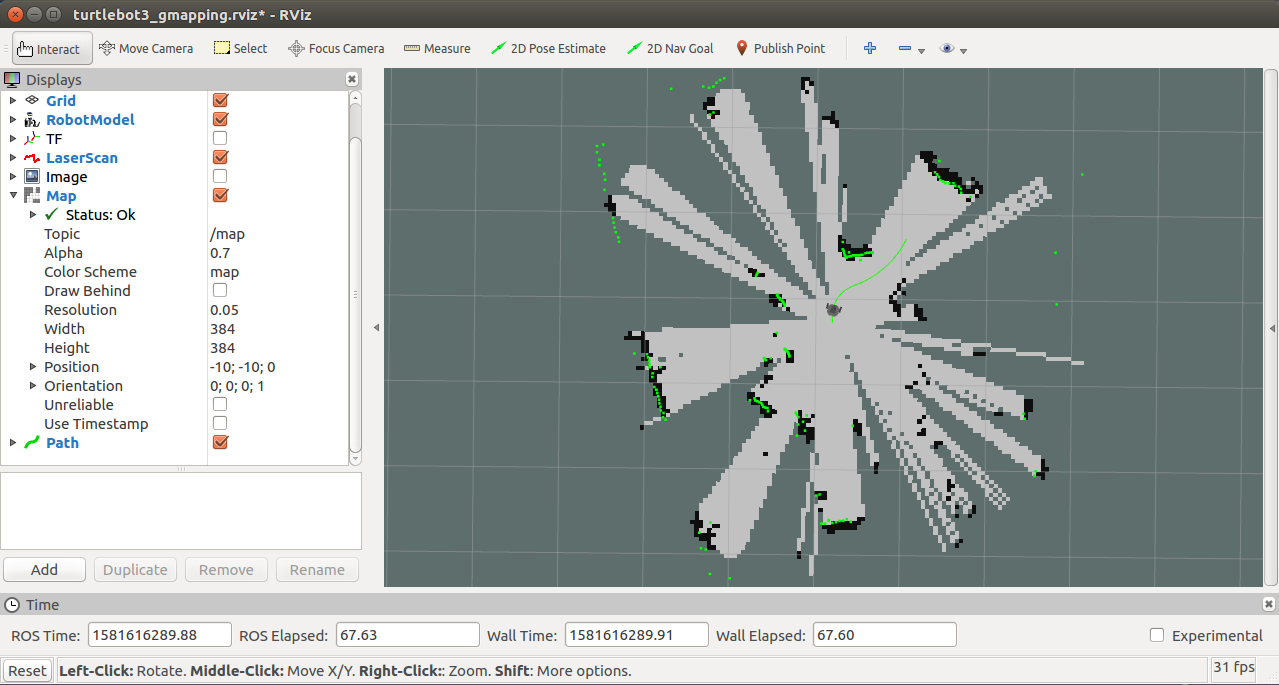
\includegraphics[width=\textwidth]{fig/4e-path.png}
		\caption{The path taken by the robot to the target point}
		\label{fig:during}
	\end{figure}

	\begin{figure}[!htb]
		\centering
		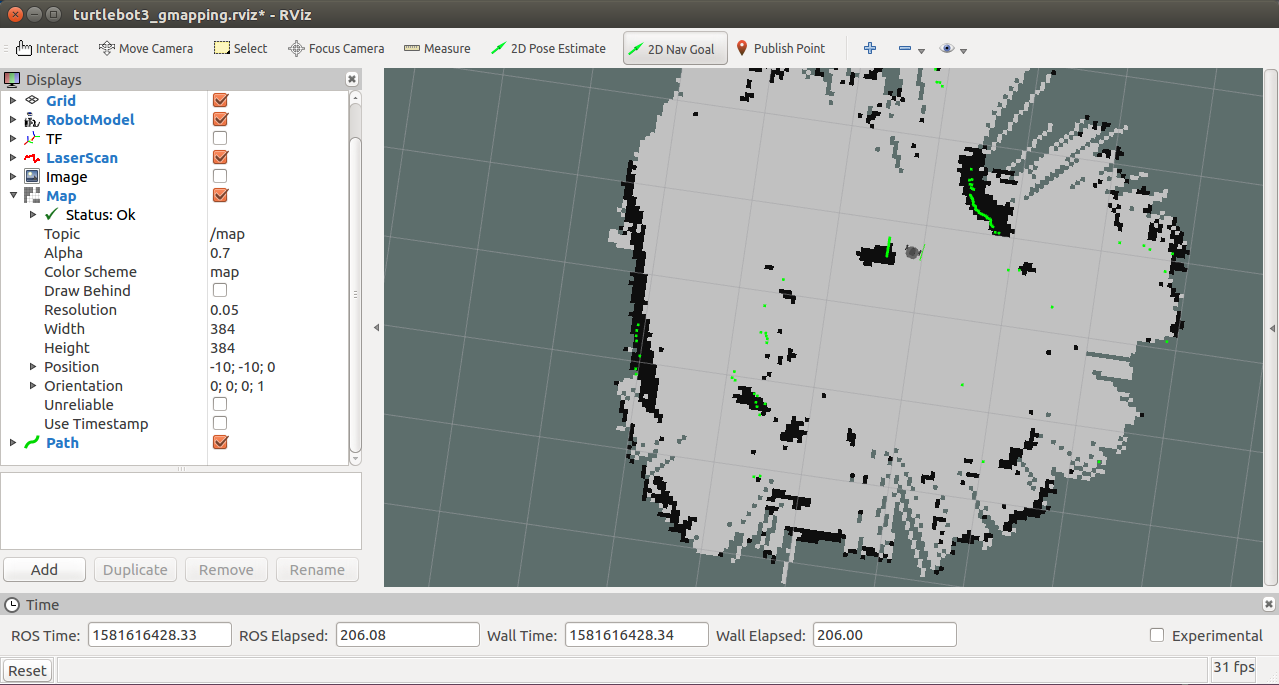
\includegraphics[width=\textwidth]{fig/4e-after.png}
		\caption{The map after the robot reaches the goal}
		\label{fig:after}
	\end{figure}
	\begin{figure}[!htb]
		\centering
		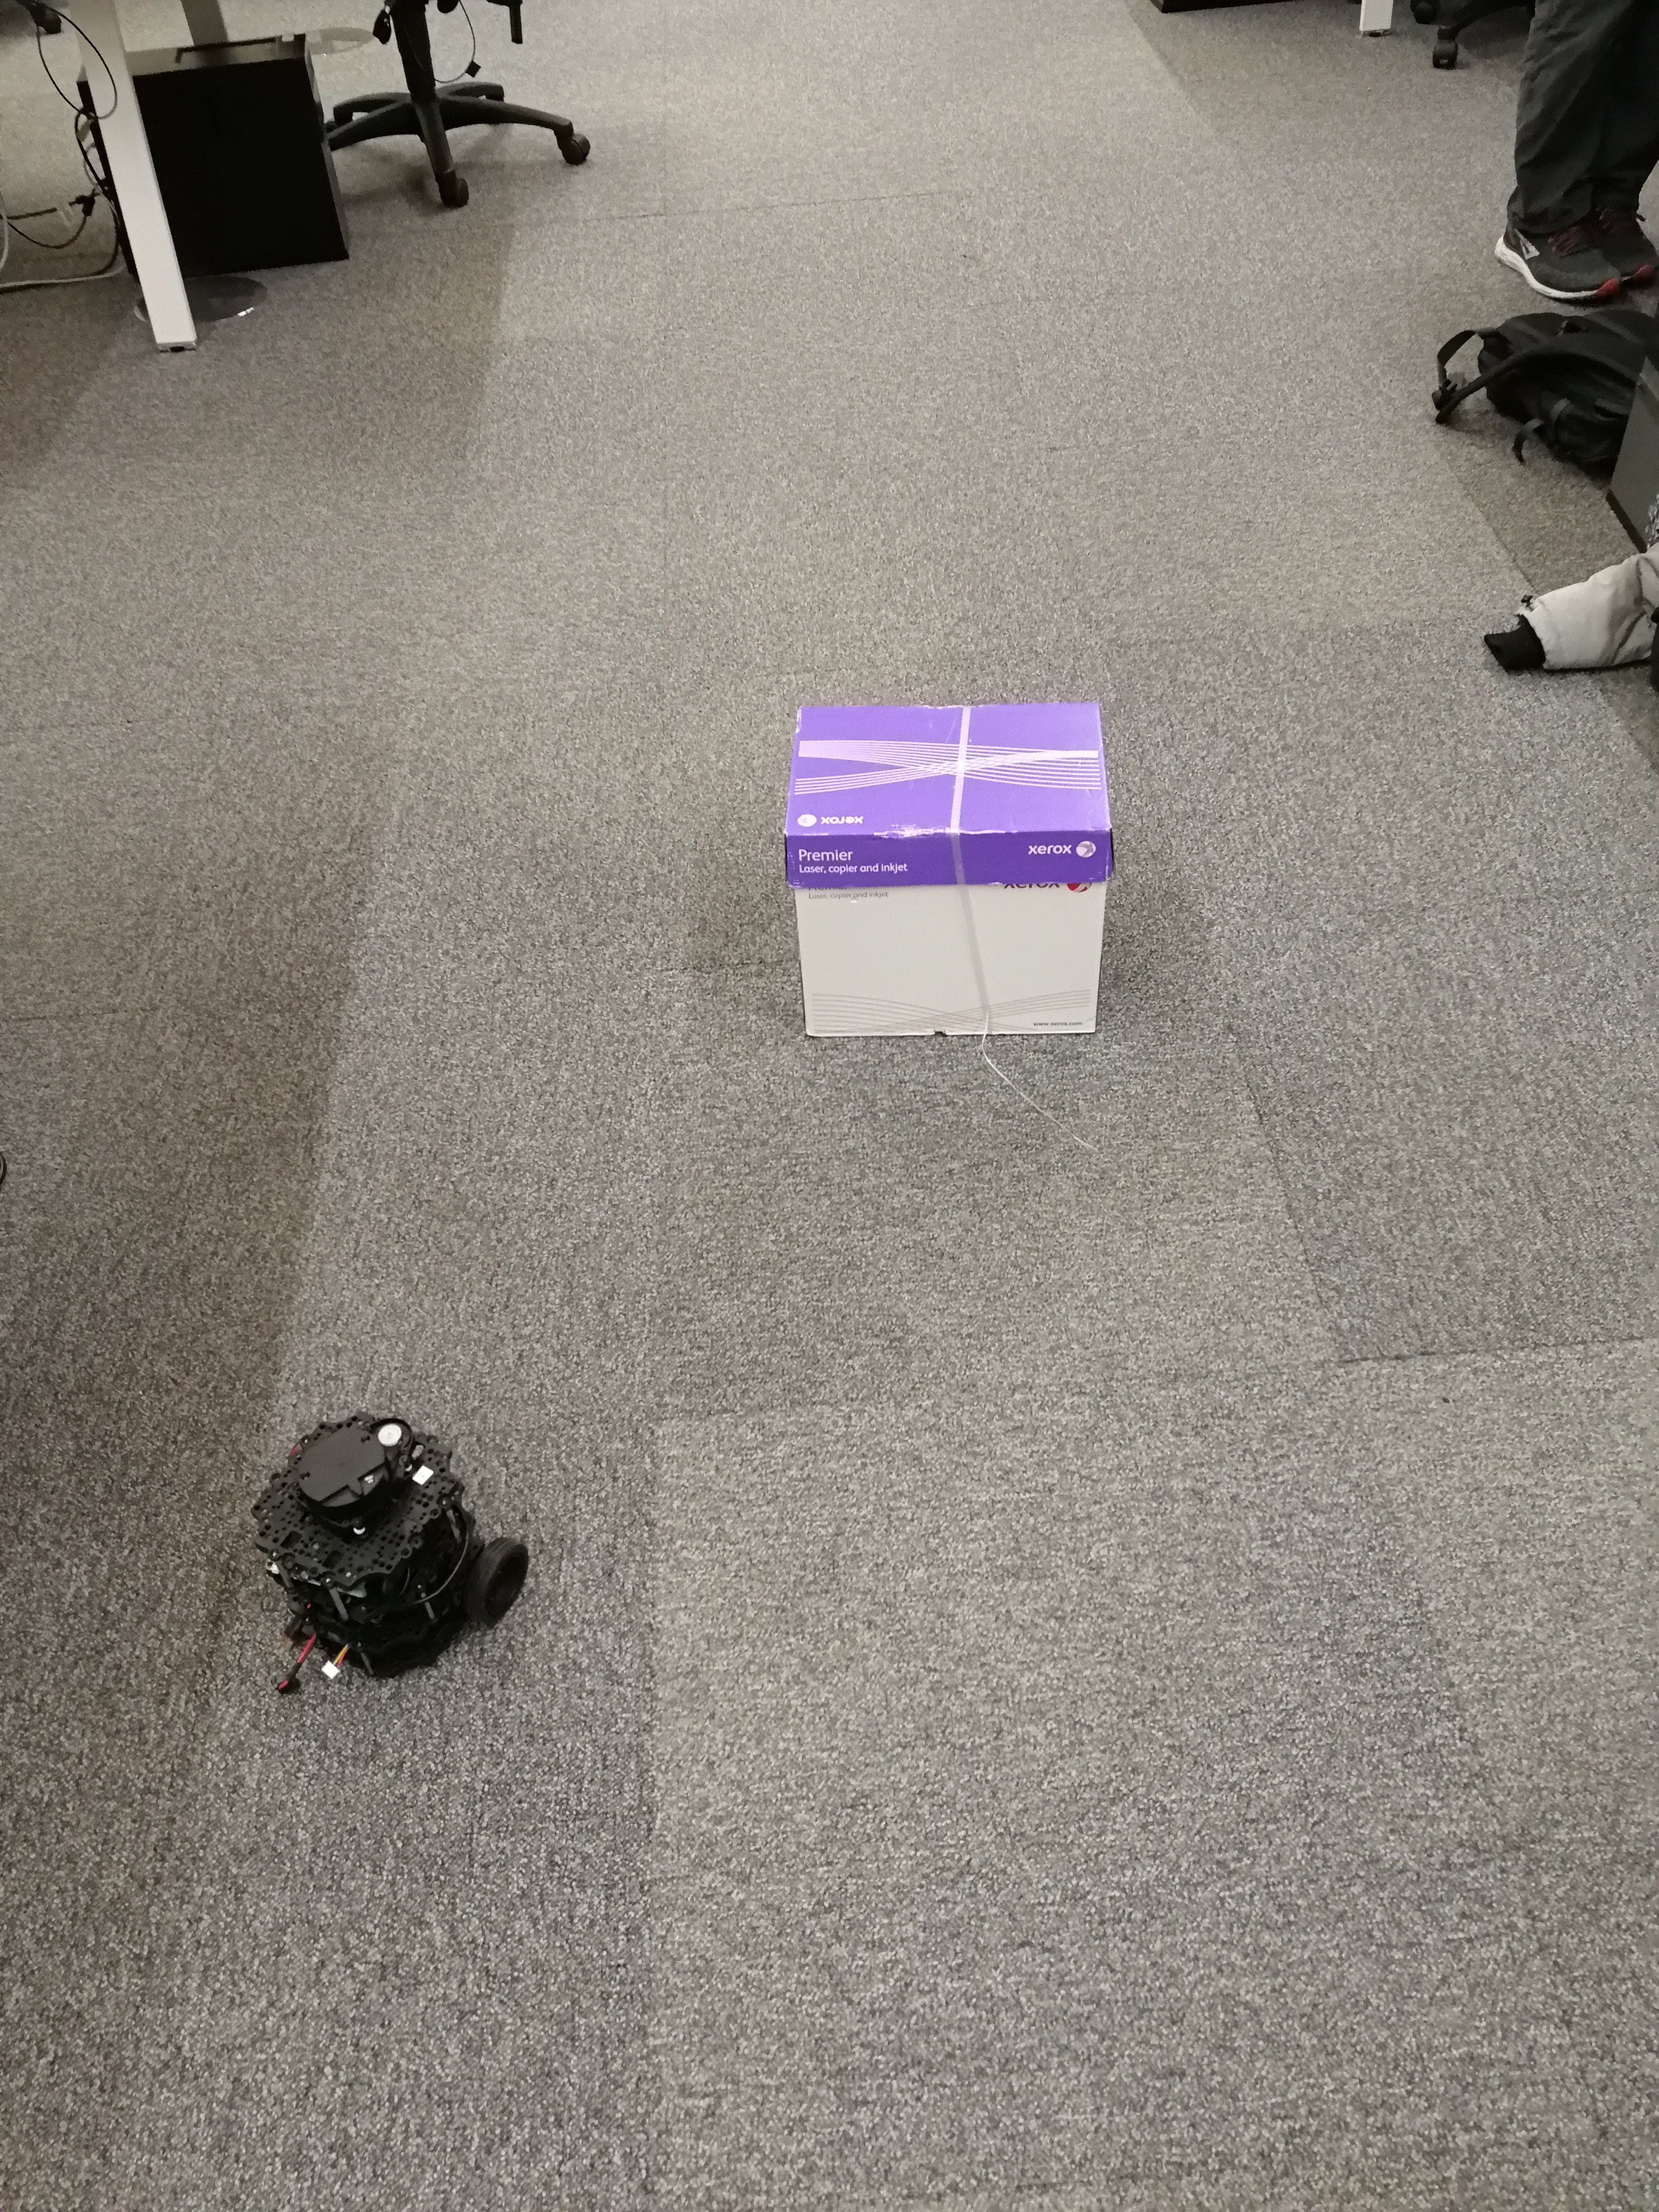
\includegraphics[width=\textwidth]{fig/4e-env.jpg}
		\caption{The environment I tested the robot in}
		\label{fig:environ}
	\end{figure}

\end{enumerate}


\end{document}
